\section{Подготовка к проведению эксперимента}

Для подготовки к программной реализации системы оценки производительности
алгоритмов оптимизации, необходимо спланировать эксперимент,
построить алгоритм проведения эксперимента, выбрать инструменты для его реализации.

\subsection{Планирование эксперимента}

Цель эксперимента — выявить преимущества и недостатки тех или иных видов
оптимизации гиперпараметров и их влияния на время обучения и производительность
модели.

Входные данные — набор текстов писем электронной почты, для каждого из которых
заранее известно, является это письмо спамом или нет.

Выходные данные — оценки нескольких обученных на входных данных классификаторов спама.

Для удобства проведения эксперимента ограничимся алгоритмами роевого интеллекта,
которые работают по общему принципу, а метод роя частиц уже показал хорошие
результаты в этой области \cite{IEEE}.

План проведения эксперимента:

\begin{itemize}
      \item[—] Выбрать наборы данных для обучения;
      \item[—] Определить набор алгоритмов для подбора параметров модели;
      \item[—] Предварительно обработать тренировочные данные;
      \item[—] Реализовать алгоритм глобальной оптимизации функции на основе того или иного природного алгоритма;
      \item[—] Выбрать оценочную функцию, подлежащую оптимизации природным алгоритмом.
            Эта функция должна вычислять оценку модели МО для каждой частицы с новыми параметрами.
            Такой функцией может служить как одна из стандартных метрик (раздел \ref{Section:Performance}), так и
            нестандартная весовая функция;
      \item[—] Получить набор параметров путем оптимизации оценочной функции; 
      \item[—] Обучить модель с использованием полученных параметров;
      \item[—] Оценить производительность полученной модели;
      \item[—] Повторить эксперимент, получив те же параметры с использованием
            других подходов к оптимизации, описанных в \ref{optimization};
      \item[—] Повторить эксперимент для других выбранных способов подбора параметров и других наборов данных;
      \item[—] Применить полученные модели к тестовым наборам данных, также провести оценку;
      \item[—] Провести сравнительный анализ получившихся оценок с целью выявления
            преимуществ и недостатков тех или иных видов оптимизации и их влияния на
            время обучения и производительность модели;
      \item[—] Объяснить полученные результаты эксперимента, сделать соответствующие выводы.
\end{itemize}

\subsubsection{Перекрестная проверка}

В данном эксперименте планируется применять перекрестную проверку как при поиске подходящих параметров, 
так и для оценки получившихся классификаторов. 

\subsubsection{Подбор параметров}

Для настройки параметров с помощью природных алгоритмов, необходимо задать число 
частиц и число популяций, а также метрику для максимизации (например, $Accuracy$). 
Затем — обучить модели с перекрестной проверкой на различных наборах
параметров, предоставляемых оптимизационным алгоритмом. Продолжать процесс 
до тех пор, пока не будет достигнуто максимальное число популяций.

\subsection{Архитектура системы для проведения эксперимента}

На Рисунке \ref{scheme} представлена блок-схема описанной системы.

\begin{figure}[H]
      \centering
      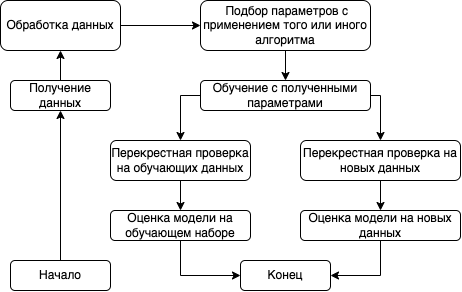
\includegraphics[width=140mm]{static/schema.png}
      \caption{Блок-схема системы для проведения эксперимента}
      \label{scheme}
\end{figure}
